% This file is part of the multi-tex ECE 486 Final Project Report 
% file name: 4-full-state-feedback-control-decoupled-observer.tex

% YOU DO NOT COMPILE FROM THIS SINGLE FILE, read the following

% included files:
% (Makefile)
% Makefile -- run make Makefile (on Mac or Linux), it takes care of LaTeX compilation

% (*.PDF)
% report.pdf -- report file, print it out and submit it

% (*.TEX)
% report.tex -- main file, pdflatex this file (tested on Mac and Linux)
% 0-title-page.tex -- title page 
% 1-introduction.tex -- chapter 1 
% 2-mathematical-model.tex -- chapter 1 (lagrange equations of motion) and chapter 4 (linearisation)
% 3-full-state-feedback-control-friction-compensation.tex -- chapter 2 and chapter 4 (two state and three state feedback controller design) 
% 4-full-state-feedback-control-decoupled-observer.tex -- (this file) chapter 4 (controller design) and chapter 5 (observer design for estimated state)
% 5-conclusions.tex -- conclusion
% 6-extra-credit.tex -- (optional) add thsese pages if you have demoed chapter 6 and chapter 7

\section{Full State Feedback Control with Decoupled Observer}

\subsection{Theoretical Background}
The observer estimates the full states of the system given the output of the system. The observers are used when there are not enough sensors or when certain system states are not directly available. Hence we use the observer to estimate the full states of the system.  In our project, we use $\delta\theta_p$ and $\delta\theta_r$ to estimate the full states of the system.
For the RWP, the system matrix is:
$$
\begin{bmatrix}
0 & 1 & 0 & 0\\
a & 0 & 0 & 0\\
0 & 0 & 0 & 1\\
0 & 0 & 0 & 0
\end{bmatrix}
$$
The top right four values and the bottom left four values of the matrix are zero. It indicates that the pendulum and rotor subsystems are independent. This special form is called the block diagonal form. This special form allows us to decouple the matrix to two 2-by-2 matrices.
$$\dot x_{1,2} = 
\begin{bmatrix}
0 & 1 \\
a & 0
\end{bmatrix}
 x_{1,2}
+
\begin{bmatrix}
0 \\
-b_p
\end{bmatrix}
u, 
C_{1,2} = 
\begin{bmatrix}
1 & 0
\end{bmatrix}
$$
$$\dot x_{3,4} = 
\begin{bmatrix}
0 & 1\\
0 & 0
\end{bmatrix}
 x_{3,4}
+
\begin{bmatrix}
0 \\
b_r
\end{bmatrix}
u, 
C_{3,4} = 
\begin{bmatrix}
1 & 0
\end{bmatrix}
$$
The advantage of decoupling the matrix is that it allows the observer response to converge quickly. It also reduces the sensitivity of the system to state variations.\\
$$
L = 
\begin{bmatrix}
l_{11} & l_{12}\\
l_{21} & l_{22}\\
l_{31} & l_{32}\\
l_{41} & l_{42}
\end{bmatrix}
$$
Since the two decoupled systems are independent, the observer dynamics are determined by $l_{11}$ , $l_{21}$ , $l_{32}$, $l_{42}$. The other terms in the 4-state observer actually make the observer to be more sensitive to model errors and noise. By decoupling the observer, we could get rid of these terms and make the observer less sensitive and making the observer more robust.
\subsection{Derivation}
The error is given by:
$$e=x-\hat{x}$$
Differentiating the equation we get:
$$\dot e=\dot x- \hat{\dot x}$$
$$\dot e=Ax+Bu-A\hat{x}-Bu-L(y-C\hat{x})$$
$$\dot e=Ax-A\hat{x}-L(Cx-C\hat{x})$$
$$\dot e=Ax-LC\hat{x}-(A\hat{x}-LC\hat{x})$$
$$\dot e=(A-LC)(x-\hat{x})$$
This is equivalent to:
$$\dot e=(A-LC)e$$
We set the poles of our observer to be [-100 -99 -98 -96] and our L matrix is:
$$
L = 
\begin{bmatrix}
196 & 1.61\\
-9637 & -159\\
-1.37 & -196\\
-135 & -9667
\end{bmatrix}
$$
At steady state $\dot e$should be equal to zero. Our A-LC matrix is:
$$
A-LC = 
\begin{bmatrix}
196 & 1 & 1.61 & 0\\
-9637 & 0 & -159 & 0\\
-1.37 & 0 & -196 & 1\\
-135 & 0 & -9667 & 0
\end{bmatrix}
$$

The poles are at: [-100 -99 -98 -96] which are all stable LHP poles.

By using Matlab, we find that the unique solution to the above matrix equation is:
$$e=
\begin{bmatrix}
0\\
0\\
0\\
0
\end{bmatrix}
$$
As such, we can see that the $e = [0 0 0 0]^T$ is the only sable equilibrium for this equation. This means that the observer states will converge to the real states over time.

\begin{figure}
  \caption{Our control block diagram of our observer feedback with friction compensation}
  \centering
    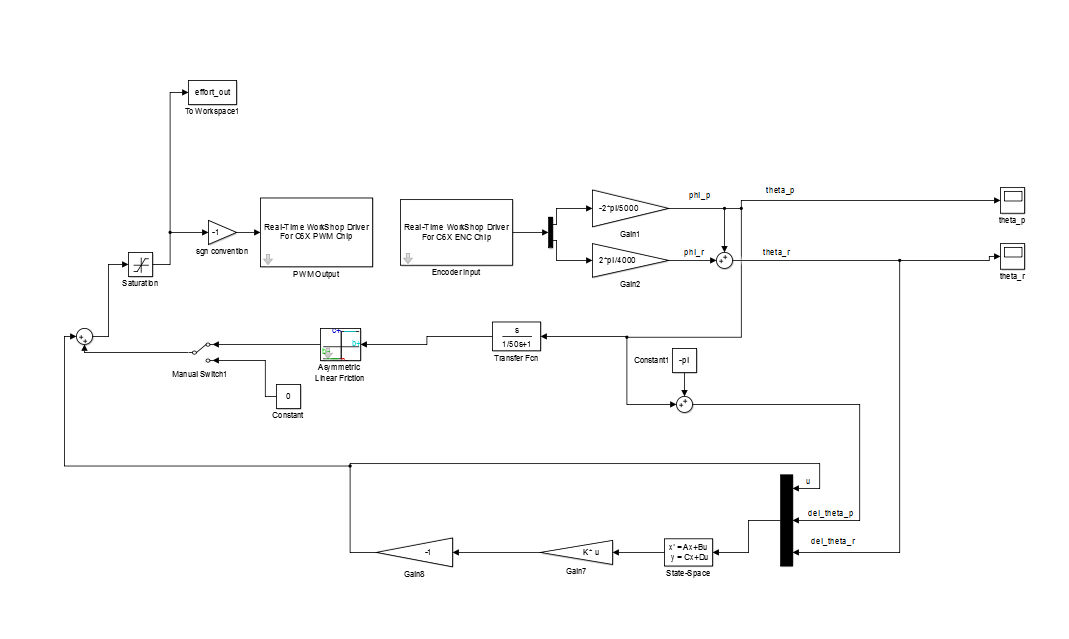
\includegraphics[scale = 0.4]{observe.PNG}
\end{figure}

\subsection{Robustness}
As shown below it's clear that our observer doesn't perform as well because it clearly can't do as well as direct access to the states.\\
\begin{tabular}{|c|c|c|c|}
\hline
 & Two-state Feedback & Three-state Feedback & Observer\\ \hline
 & $\delta\theta_p$  $\delta\theta_r$ & $\delta\theta_p$  $\delta\theta_r$ & $\delta\theta_p$  $\delta\theta_r$\\ \hline
Max IC deviations & 0.12  1.1 & 0.12  1 & 0.12  0.99\\ \hline
Max pulse & 7.5 & 8.1 & 7\\ \hline
Max disturbance & 5 & 7.4 & 6.3\\
\hline
\end{tabular}
\subsection{System Behavior}
The observer approach could also stabilize the system at the equilibrium point. The observer design has higher sensitivity than the full-state design meaning that the observer design could only reject smaller pulse, constant disturbances than the full-state controller. This means that the observer feedback controller is not as robust as the full-state feedback controller. The observer design has higher sensitivity since it could only estimate the approximate values of the states of the system.